% !TeX spellcheck = fr_FR
\chapter{Chapitre 1 : Données et formats}

% \begin{center}
% 	\textit{Chaque chapitre doit commencer sur une nouvelle page.}\\*[35pt]
% \end{center}

Dans ce chapitre nous allons aborder les différents format de données qui seront
cités dans la suite de ce document.

\section{Données LIDAR}

LIDAR veut dire << Light Detection And Ranging >> ou en français 
<< détection et estimation de la distance par la lumière >>. 
Il s’agit d’une technique de mesure de distance où la lumière réalise un 
aller-retour entre sa source et un objet. On chronomètre le temps entre le moment 
où une pulsation de lumière est émise par un laser et son retour vers un capteur.
En connaissant la vitesse de propagation de la lumière dans l’environnement où
évolue la lumière, il est possible de déterminer la distance qui sépare l’objet 
du capteur. Plus précisément il s’agit de la distance  séparant l'instrument de
mesure et un point de l’objet frapé par la lumière émise. 
Cette opération effectuée à de multiple reprise en changeant par petit pas 
l’angle du laser crée d’autres points qui une fois réunis 
constituent un nuage de points profilant l'environnement autour de l'instrument.
Si l'instrument de mesure est placé sur un avion et que la source de lumière est
dirigé vers le bas, il est ainsi possible de capturer, sous forme d'un nuage de
points, une région du globe. Ce cas nécessite tout de fois de connaître la position
GPS de l'avion au moment de la capture d'un point afin de mettre en relation
tous les points à la fin de la mesure.

\subsection{Format de données LAS}

le format de stockage des nuages de points de données LIDAR, est un format
binaire dont les spécifications sont érigées par <mettre le nom ici>

% \begin{figure}[tbph!]
% 	\centering
% 	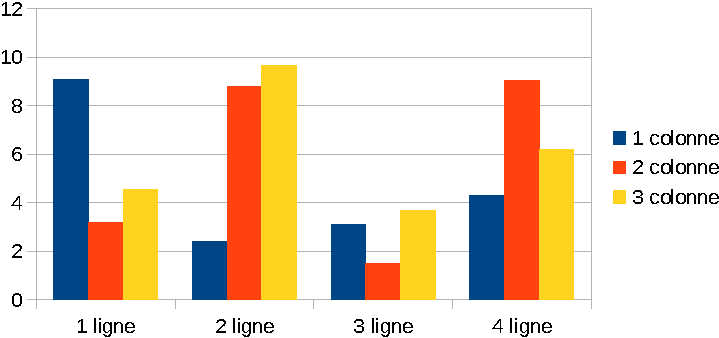
\includegraphics[width=0.7\linewidth]{chart}
% 	\caption[Diagramme machin]{Diagramme machin. Source : tiré de Tartempion 2010, p. 42 / tiré de ce-site.ch, ref. URL01 / réalisé par Nom Prénom.}
% 	\label{fig:chart1}
% \end{figure}
% 
% 
% \begin{table}[tbph!]
% 	\centering{
% 		\begin{tabular}{ |l|c|c|c| }
% 			\hline
% 			& \textbf{Condition 1} & \textbf{Condition 2} & \textbf{Condition 3} \\
% 			\hline
% 			\textbf{Test 1} & X & O & X \\
% 			\hline
% 			\textbf{Test 2} & O & X & X \\
% 			\hline
% 			\textbf{Test 3} & O & X & O \\
% 			\hline 
% 		\end{tabular}
% 		\caption[Lot de données n°1]{Lot de données n°1. Source: tiré de Tartempion 2010, p. 42 / tiré de ce-site.ch, ref. URL02 / réalisé par Nom Prénom.}
% 		\label{tab:tableau1}
% 	}
% \end{table}
% 
% 
% \begin{figure}[tbph!]
% 	\centering
% 	
\includegraphics[width=0.7\linewidth]{diagram}
% 	\caption[Schéma bidule.]{Schéma bidule. Source : tiré de Tartempion 2010, p. 42 / tiré de ce-site.ch, ref. URL03 / réalisé par Nom Prénom.}
% 	\label{fig:diagram}
% \end{figure}
% 
% 
% \section{Titre de niveau 2}
% 
% 
% \begin{figure}[tbph!]
% 	\centering
% 	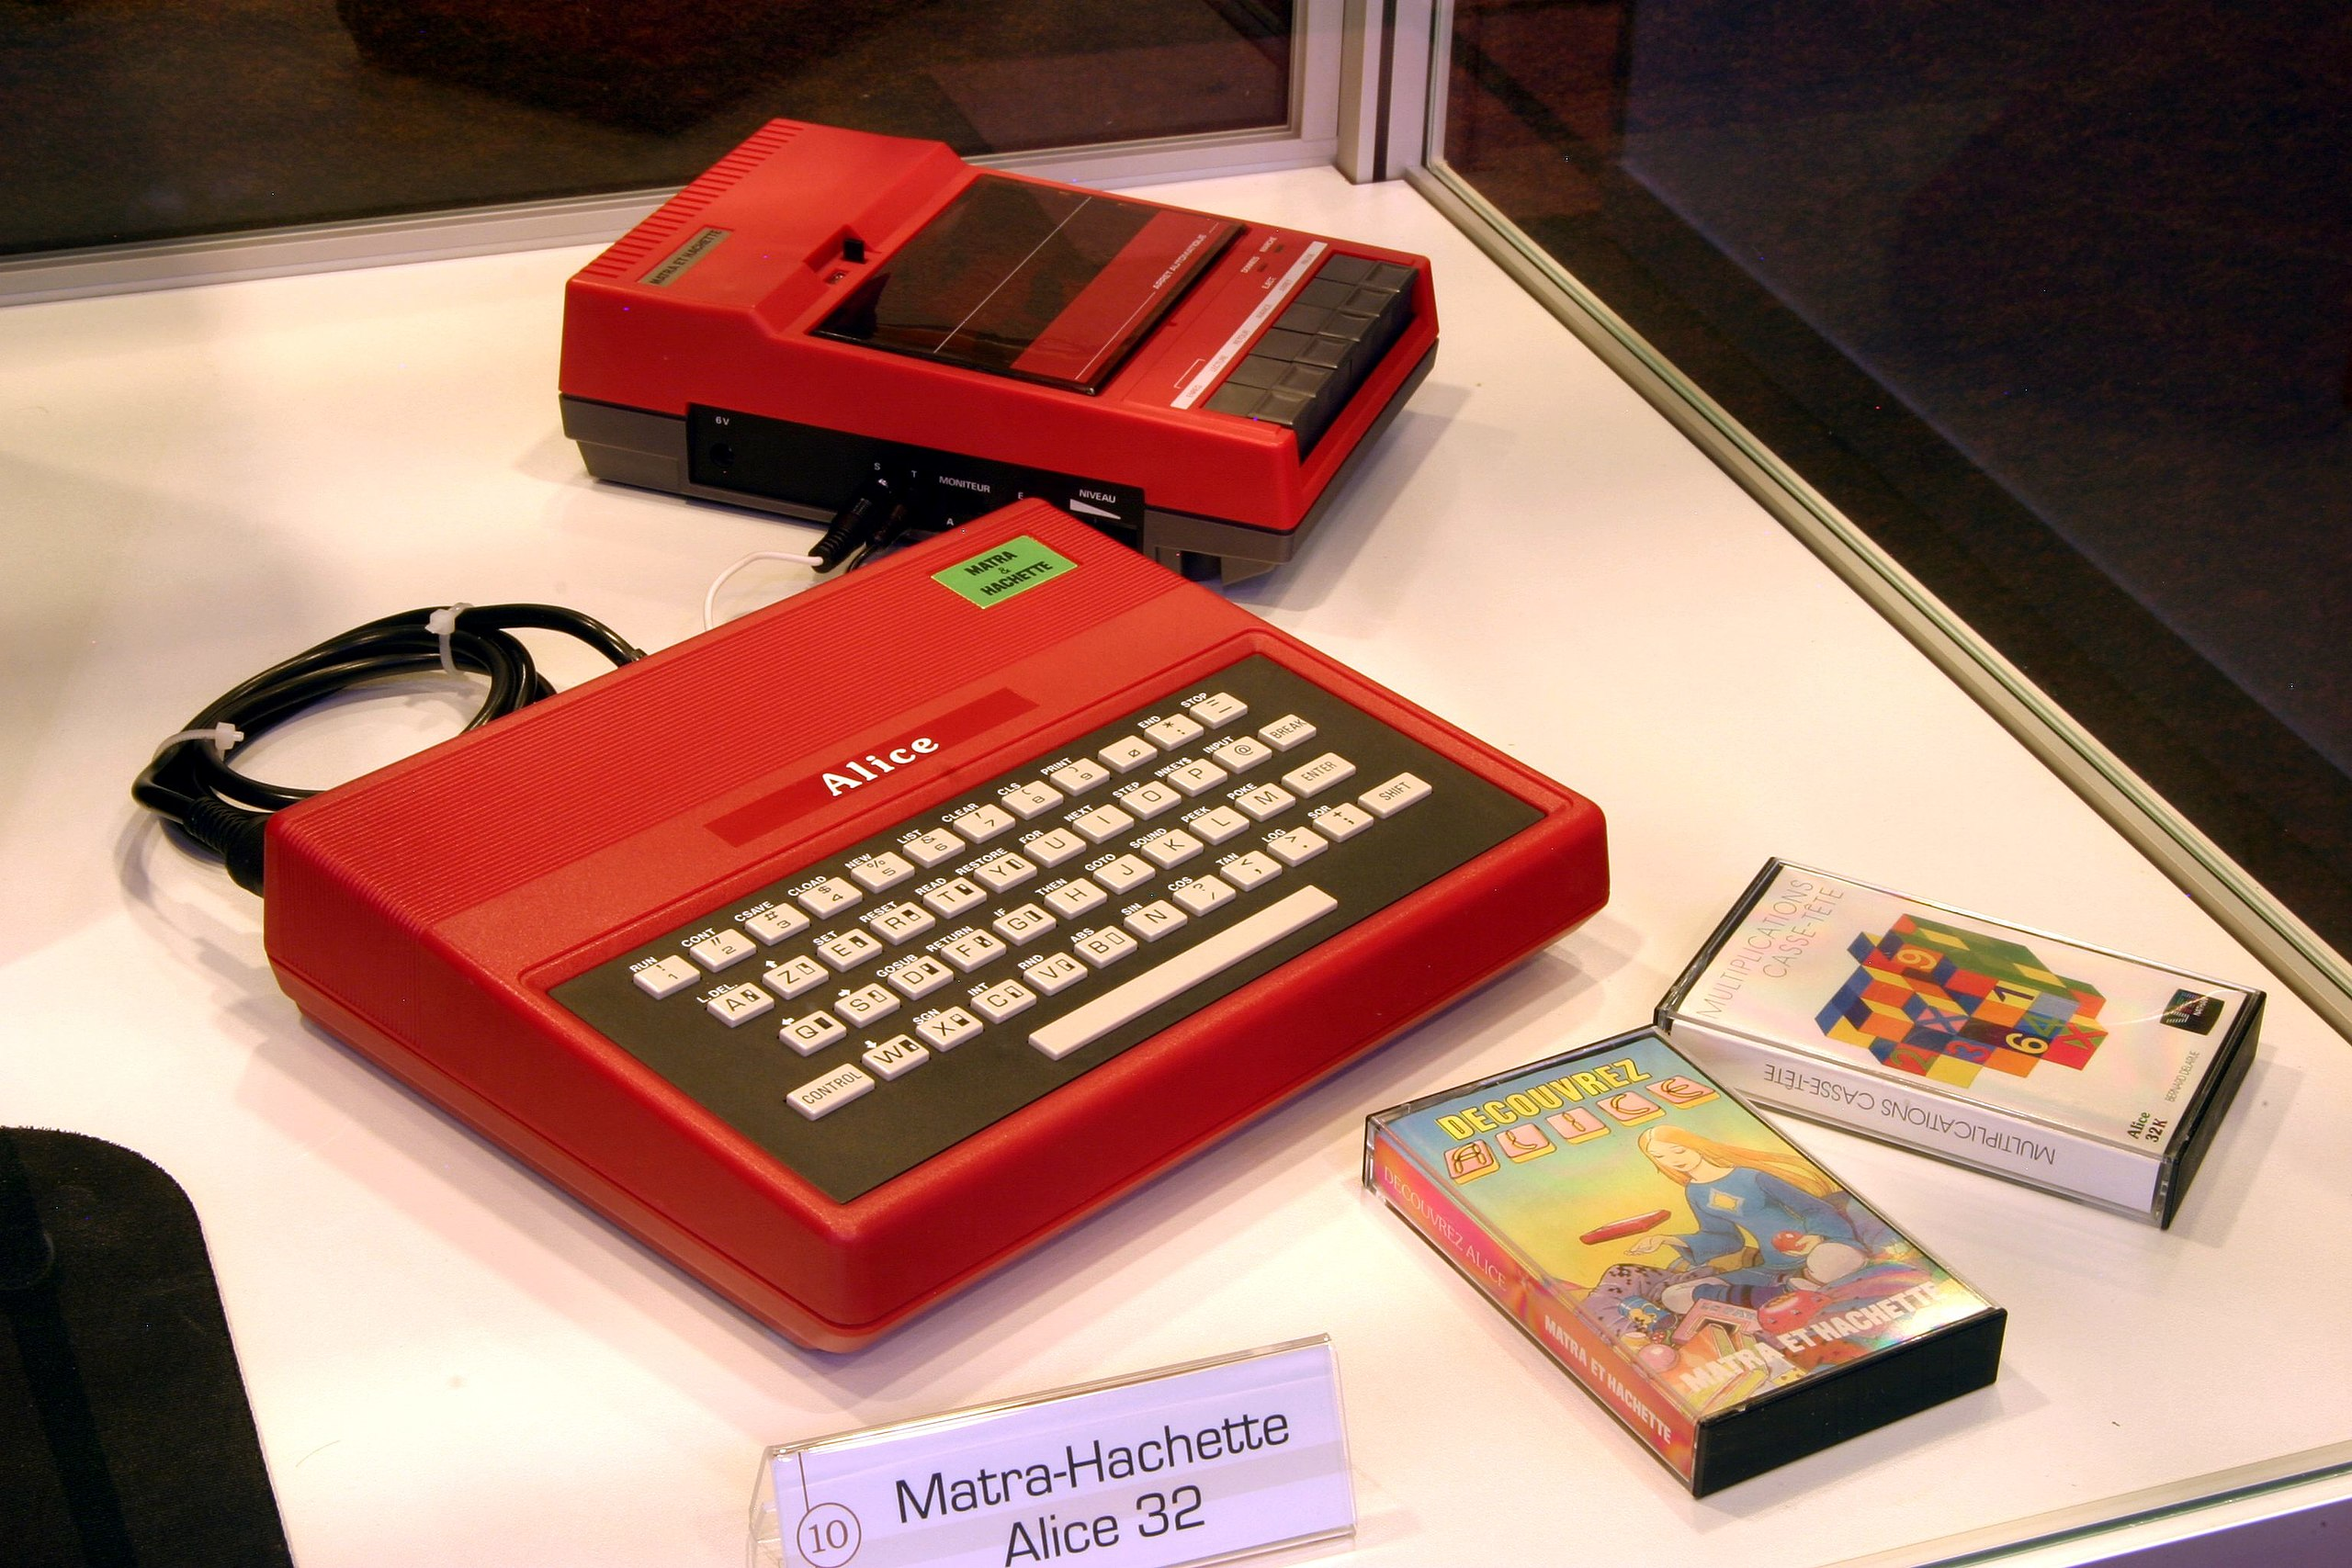
\includegraphics[width=0.7\linewidth]{ordi}
% 	\caption[Alice, Micro-ordinateur MATRA.]{Alice, Micro-ordinateur MATRA. Source : tiré de Tartempion 2010, p. 42 / tiré de ce-site.ch, ref. URL03 / réalisé par Nom Prénom.}
% 	\label{fig:image}
% \end{figure}
% 
% 
% \subsection{Titre de niveau 3}
% 
% 
% \begin{table}[tbph!]
% 	\centering{
% 		\begin{tabular}{ |l|c|c|c| }
% 			\hline
% 			& \textbf{Condition 1} & \textbf{Condition 2} & \textbf{Condition 3} \\
% 			\hline
% 			\textbf{Test 1} & X & O & X \\
% 			\hline
% 			\textbf{Test 2} & O & X & X \\
% 			\hline
% 			\textbf{Test 3} & O & X & O \\
% 			\hline 
% 		\end{tabular}
% 		\caption[Lot de données n°2.]{Lot de données n°2. Source: tiré de Tartempion 2010, p. 42 / tiré de ce-site.ch, ref. URL05 / réalisé par Nom Prénom.}
% 		\label{tab:tableau2}
% 	}
% \end{table}
